%%%%%%%%%%%%%%%%%%%%%%%%%%% asme2e.tex %%%%%%%%%%%%%%%%%%%%%%%%%%%%%%%
% Template for producing ASME-format articles using LaTeX            %
% Written by   Harry H. Cheng                                        %
%              Integration Engineering Laboratory                    %
%              Department of Mechanical and Aeronautical Engineering %
%              University of California                              %
%              Davis, CA 95616                                       %
%              Tel: (530) 752-5020 (office)                          %
%                   (530) 752-1028 (lab)                             %
%              Fax: (530) 752-4158                                   %
%              Email: hhcheng@ucdavis.edu                            %
%              WWW:   http://iel.ucdavis.edu/people/cheng.html       %
%              May 7, 1994                                           %
% Modified: February 16, 2001 by Harry H. Cheng                      %
% Modified: January  01, 2003 by Geoffrey R. Shiflett                %
% Use at your own risk, send complaints to /dev/null                 %
%%%%%%%%%%%%%%%%%%%%%%%%%%%%%%%%%%%%%%%%%%%%%%%%%%%%%%%%%%%%%%%%%%%%%%

%%% use twocolumn and 10pt options with the asme2e format
\documentclass[cleanfoot,cleanhead,twocolumn,10pt,notitlepage]{asme2e}
\special{papersize=8.5in,11in}

\usepackage{listings}
\usepackage{graphicx}
\usepackage{amsmath}
\usepackage[hidelinks]{hyperref}
\lstset{
    breaklines=true, % break lines for files
    basicstyle=\scriptsize,
    numbers=left,
    showstringspaces=false,
    frame=l
}

%% The class has several options
%  onecolumn/twocolumn - format for one or two columns per page
%  10pt/11pt/12pt - use 10, 11, or 12 point font
%  oneside/twoside - format for oneside/twosided printing
%  final/draft - format for final/draft copy
%  cleanfoot - take out copyright info in footer leave page number
%  cleanhead - take out the conference banner on the title page
%  titlepage/notitlepage - put in titlepage or leave out titlepage
%  
%% The default is oneside, onecolumn, 10pt, final

%%% You need to remove 'DRAFT: ' in the title for the final submitted version.
\title{Major Project \# 2}

%%% first author
\author{Shaun Harris
    \affiliation{
	Department of Mechanical and Aerospace Engineering\\
	Utah State University \\
    Email: shaun.r.harris@gmail.com
    }
}


\begin{document}

\maketitle    

%%%%%%%%%%%%%%%%%%%%%%%%%%%%%%%%%%%%%%%%%%%%%%%%%%%%%%%%%%%%%%%%%%%%%%

\begin{abstract}
    {\it The solid motor propulsion rates for a small ``Pike" missile was simulated.  The chamber pressure, regression rate, massflow, choked massflow, mass depletion, thrust profile, and $I_{sp}$ was analyzed for cylindrical port burning and for Bates grain burning.}
\end{abstract}


\tableofcontents

%%%%%%%%%%%%%%%%%%%%%%%%%%%%%%%%%%%%%%%%%%%%%%%%%%%%%%%%%%%%%%%%%%%%%%

\begin{nomenclature}
    \entry{$L_0,L_{port}$} {Total length of propellant}
    \entry{$D_0$} {Outer diameter of propellant}
    \entry{$d_0$} {Inner diameter of propellant}
    \entry{$\rho,\rho_{propellant}$} {density of propellant}
    \entry{$A^*$}{Throat area}
    \entry{$A_{exit}$}{Nozzle exit area}
    \entry{$M_W$}{Molecular weight}
    \entry{$T_0$}{Flame temperature}
    \entry{$a,n,M_{crit,k}$}{properties for calculating $\dot{r}$}
    \entry{$\dot{r}$}{Linear change of propellant per time in direction perpendicular to surface}
    \entry{$\dot{P_0}$}{Change in chamber pressure per time}
    \entry{$r$}{Inner radius of solid propellant}
    \entry{$P_0$}{Chamber pressure}
    \entry{$t$}{time in seconds}
\end{nomenclature}

\section{INTRODUCTION}

A small missle was simulated using the erosive and bates grain burning methods.  Two simulations were run and compared.  The first was a cylindrical port simulation, where erosive burning was used.  The second simulation used three individual blocks of bates grains where the ends were not burn inhibited.  It also did not use erosive burning.  Many of the properties were shared.  Eq. \ref{eq:shared} shows the shared properties.  The first simulation had a specific $k=0.2$ and the second simulation set $k=0$ to neglect the erosive burning.  Eq. \ref{eq:part1} shows the relevant equations for the first simulation and Eq. \ref{eq:part2} shows the relevant equations for the second simulation.

\begin{equation}
\begin{aligned}
    L_0 &= 35 cm \\
    D_0 &= 6.6 cm\\
    d_0 &= 3 cm\\
    \rho &= 1260 \frac{kg}{m^3}\\
    A^* &= 1.887 cm^2 \\
    \frac{A_{exit}}{A^*} &= 4.0 \\
    \theta_{exit} &= 20 deg \\
    \gamma &= 1.18 \\
    M_W &= 23 \frac{kg}{kg-mol}\\
    T_0 &= 2900 K\\
    a &= 0.132 \frac{cm}{s-kPa^n}\\
    n &= 0.16 \\
    M_{crit} &= 0.3
\label{eq:shared}
\end{aligned}
\end{equation}

\begin{equation}
\begin{aligned}
    \dot{P_0} &= \frac{A_{burn} \dot{r}}{V_c} 
        \left( \rho_{propellant} R_g T_0 - P_0 \right) P_0 \sqrt{\gamma R_g T_0 
        \left( \frac{2}{\gamma + 1}\right)^{\frac{\gamma+1}{\gamma-1}}} \\
    \dot{r} &= a P_0^n\\
    P_0 &= P_{ambient} \\
    r &= \frac{d_0}{2} \\ 
    A_{burn} &= 2 \pi r L_{port} \\
    V_c &= \pi r^2 L_{port} 
\label{eq:part1}
\end{aligned}
\end{equation}

\begin{equation}
\begin{aligned}
    \dot{P_0} &= \frac{A_{burn} \dot{r}}{V_c} 
        \left( \rho_{propellant} R_g T_0 - P_0 \right) P_0 \sqrt{\gamma R_g T_0 
        \left( \frac{2}{\gamma + 1}\right)^{\frac{\gamma+1}{\gamma-1}}} \\
    \dot{r} &= a P_0^n \left( \frac{1+k\frac{M_{port}}{M_crit}}{1+k} \right) \\
    P_0 &= P_{ambient} \\
    r &= \frac{d_0}{2} \\ 
    A_{burn} &= N \pi \left[ \frac{D_0^2-(d_0+2 s)^2}{2} + (L_0 - 2 s)(d_0 + 2 s)\right]\\
    V_c &= \frac{N \pi}{4} \left[ (d_0 + 2 s)^2 (L_0 - 2 s) + D_0^2 2 s \right]
\label{eq:part2}
\end{aligned}
\end{equation}


\section{RESULTS}

Each simulation had their own set of results.  The subsections below will outline the results for each.

\subsection{Part 1 Cylindrical Port with Erosive burning}

The following figures outline the results for each of the quantities of interest.

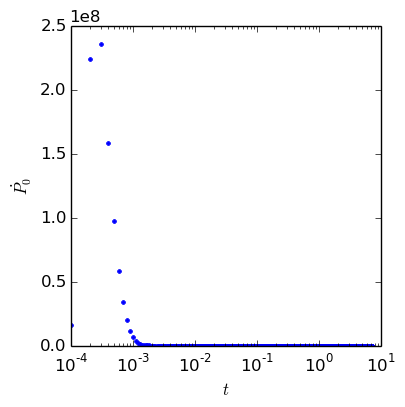
\includegraphics[width=\linewidth]{../python_stuff/Part1/P0_dot.png}

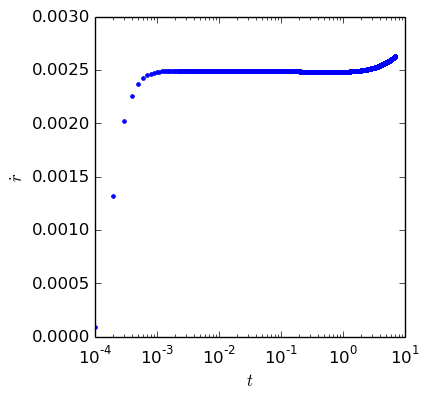
\includegraphics[width=\linewidth]{../python_stuff/Part1/r_dot.png}

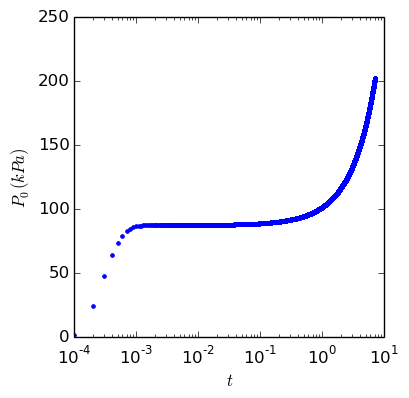
\includegraphics[width=\linewidth]{../python_stuff/Part1/P0.png}

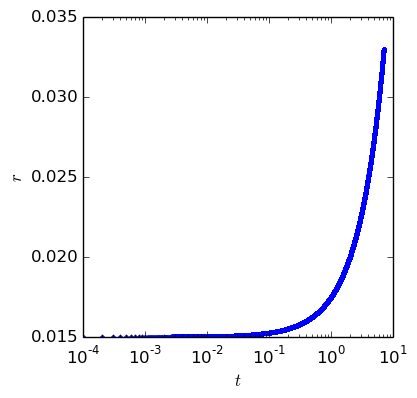
\includegraphics[width=\linewidth]{../python_stuff/Part1/r.png}

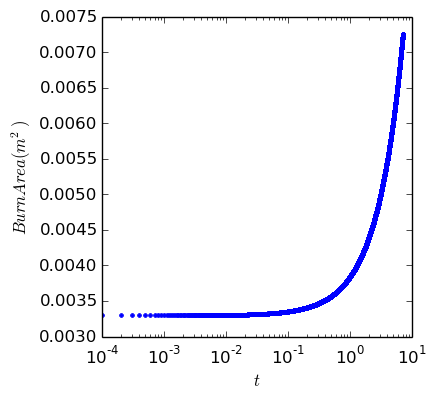
\includegraphics[width=\linewidth]{../python_stuff/Part1/BurnArea.png}

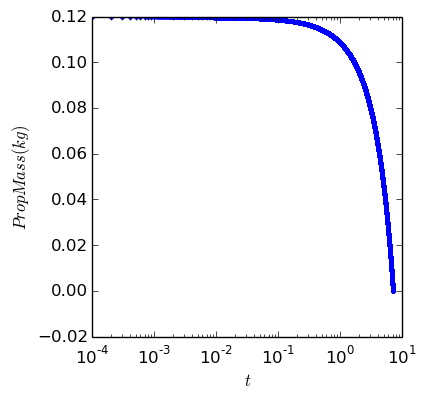
\includegraphics[width=\linewidth]{../python_stuff/Part1/PropMass.png}

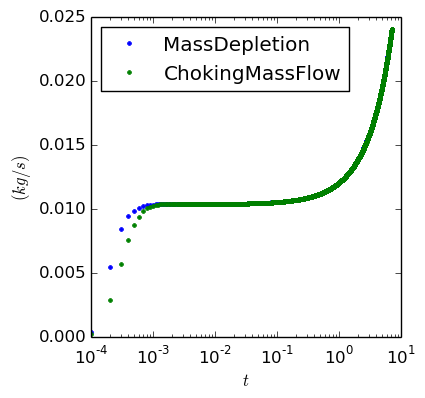
\includegraphics[width=\linewidth]{../python_stuff/Part1/MassFlows.png}

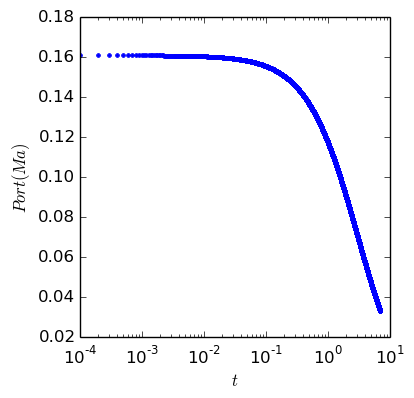
\includegraphics[width=\linewidth]{../python_stuff/Part1/PortMach.png}

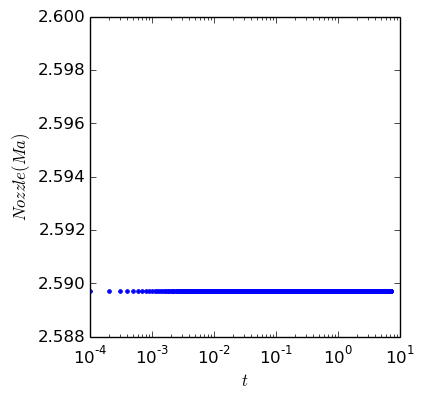
\includegraphics[width=\linewidth]{../python_stuff/Part1/NozzMach.png}

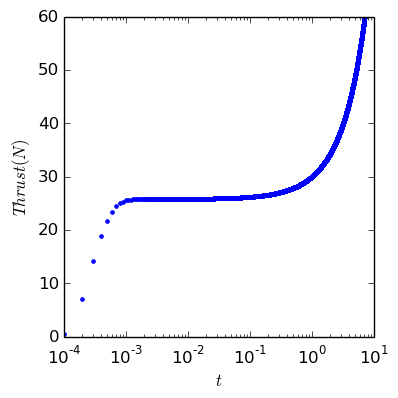
\includegraphics[width=\linewidth]{../python_stuff/Part1/Thrust.png}

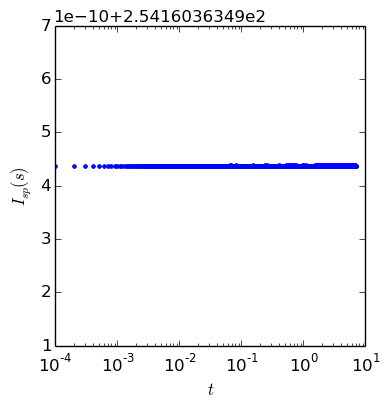
\includegraphics[width=\linewidth]{../python_stuff/Part1/Isp.png}

Where the effective mean $I_{sp}=254.16 s$.


\subsection{Part 2 Bates grain with non-erosive burning}

The following figures outline the results for each of the quantities of interest.

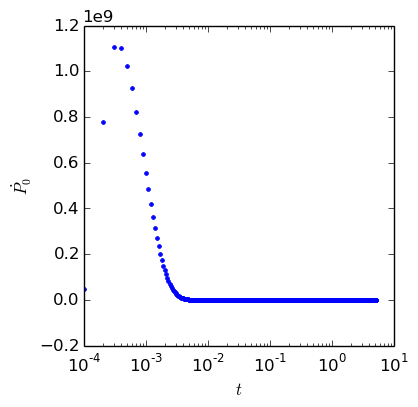
\includegraphics[width=\linewidth]{../python_stuff/Part2/P0_dot.png}

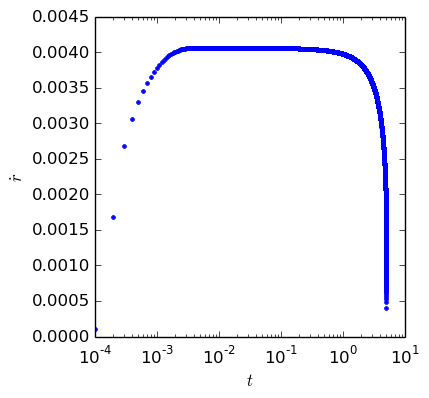
\includegraphics[width=\linewidth]{../python_stuff/Part2/r_dot.png}

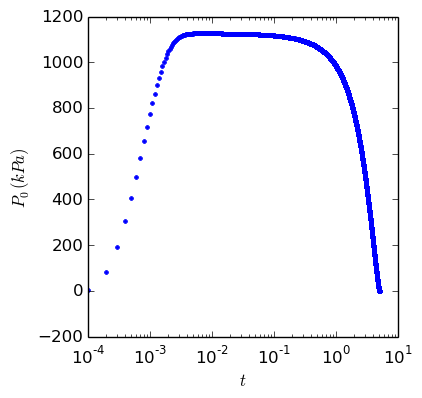
\includegraphics[width=\linewidth]{../python_stuff/Part2/P0.png}

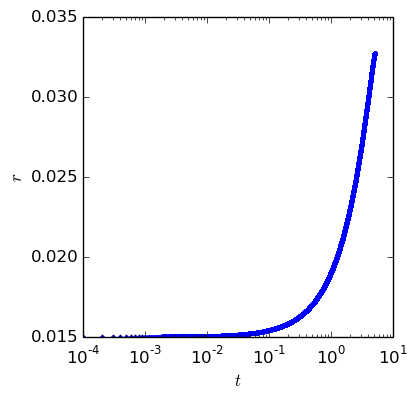
\includegraphics[width=\linewidth]{../python_stuff/Part2/r.png}

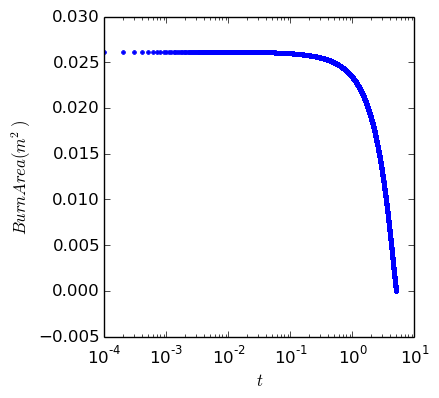
\includegraphics[width=\linewidth]{../python_stuff/Part2/BurnArea.png}

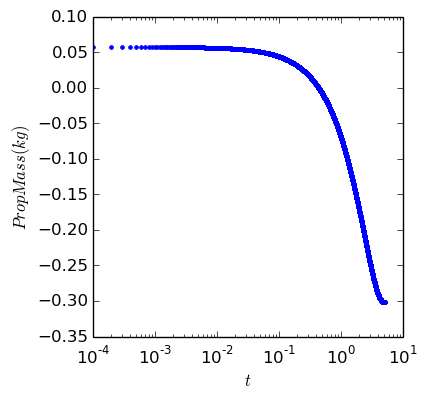
\includegraphics[width=\linewidth]{../python_stuff/Part2/PropMass.png}

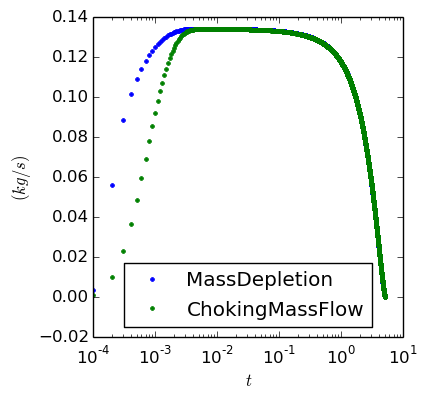
\includegraphics[width=\linewidth]{../python_stuff/Part2/MassFlows.png}

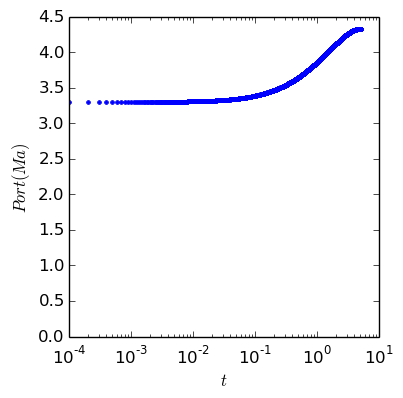
\includegraphics[width=\linewidth]{../python_stuff/Part2/PortMach.png}

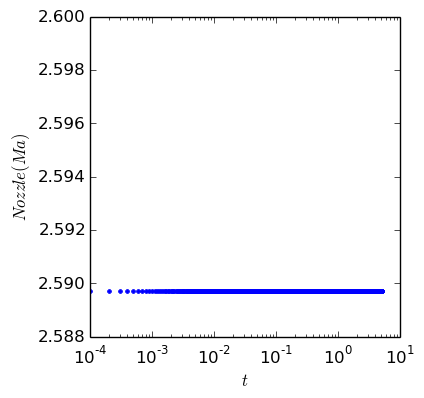
\includegraphics[width=\linewidth]{../python_stuff/Part2/NozzMach.png}

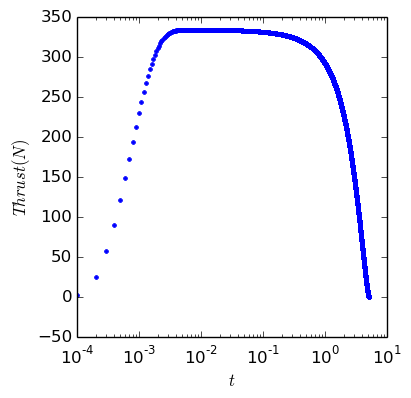
\includegraphics[width=\linewidth]{../python_stuff/Part2/Thrust.png}

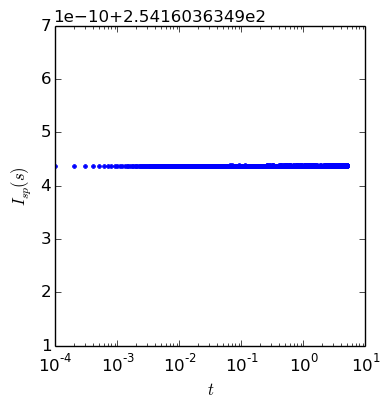
\includegraphics[width=\linewidth]{../python_stuff/Part2/Isp.png}

Where the effective mean $I_{sp}=254.16 s$.

\subsection{Sensitivity and effect of flame temperature}

In addition to the above plots, analysis was run to see the sensitivity of the input parameters.  It was found that small changes can lead to large changes in the output values.  Thus, care must be taken to ensure correct and repeatable parameters are provided for rockets. For example, by changing $T_0 = 3300$ we can compare the two plots of $P_0$ vs time to see the change in the values.  It is fairly drastic.  

This is the original $P_0$ plot shown above in Part 2.  

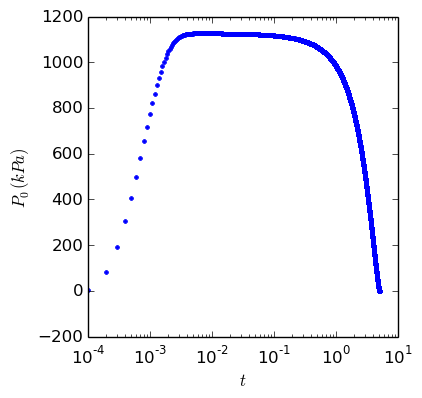
\includegraphics[width=\linewidth]{../python_stuff/Part2/P0.png}

This is the value of $P_0$ with the increased flame temperature.

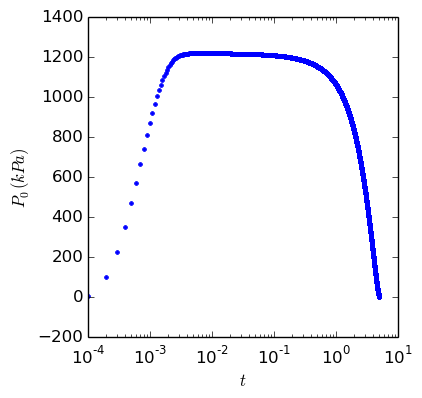
\includegraphics[width=\linewidth]{../python_stuff/Part2_flameTemp/P0.png}

Additionally, the regression vs chamber pressure was shown in this next plot.

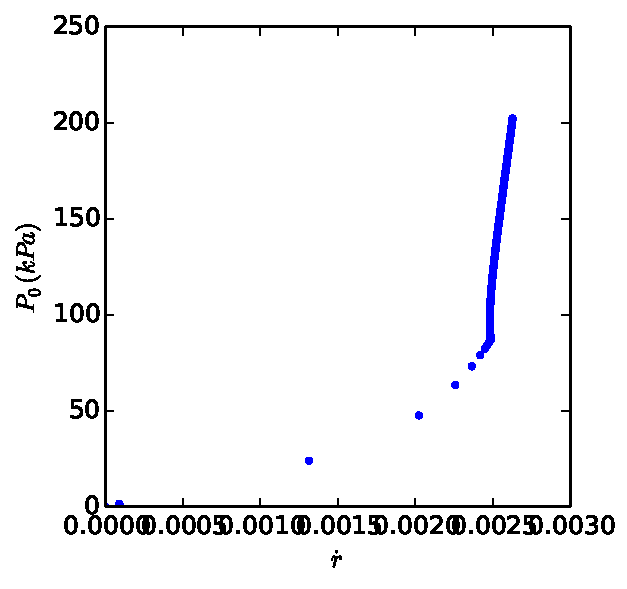
\includegraphics[width=\linewidth]{../python_stuff/Part1/Reg_v_P0.pdf}

%%%%%%%%%%%%%%%%%%%%%%%%%%%%%%%%%%%%%%%%%%%%%%%%%%%%%%%%%%%%%%%%%%%%%%

\section{CONCLUSION}

These calculations used compressible fluid flow as well as solid propellant simulations.  We were able to show the many quantities of interest for the two situations.  


%%%%%%%%%%%%%%%%%%%%%%%%%%%%%%%%%%%%%%%%%%%%%%%%%%%%%%%%%%%%%%%%%%%%%%

%\bibliographystyle{asmems4}
%\bibliography{asme2e}

%%%%%%%%%%%%%%%%%%%%%%%%%%%%%%%%%%%%%%%%%%%%%%%%%%%%%%%%%%%%%%%%%%%%%%

%
%%%%%%%%%%%%%%%%%%%%%%%%%%%%%%%%%%%%%%%%%%%%%%%%%%%%%%%%%%%%%%%%%%%%%%
%\clearpage

\appendix

\section{Appendix A: Code}
\label{sec:code}
\subsection*{Header files}
\lstinputlisting[language=c++]{../cpp_stuff/DEFS.h}
\lstinputlisting[language=c++]{../cpp_stuff/Prandtl_Meyer.h}
\lstinputlisting[language=c++]{../cpp_stuff/CylindricalPort.h}
\lstinputlisting[language=c++]{../cpp_stuff/RP.h}
\lstinputlisting[language=c++]{../cpp_stuff/Solver.h}
\subsection*{Linked c\texttt{++} files}
\lstinputlisting[language=c++]{../cpp_stuff/Prandtl_Meyer.cpp}
\lstinputlisting[language=c++]{../cpp_stuff/CylindricalPort.cpp}
\lstinputlisting[language=c++]{../cpp_stuff/RP.cpp}
\lstinputlisting[language=c++]{../cpp_stuff/Solver.cpp}
\subsection*{Main Program}
\lstinputlisting[language=c++]{../cpp_stuff/Project2.cpp}





\end{document}
